\section{Trapezregel}
\label{sec:trapezregel}
Diese brauche wir zur numerischen Integration, beipielweise um Warscheinlichkeit in einer Normalverteilung zu berechnen. Diese Integrale können, wie in \autoref{sec:statistische_grundlagen} besprochen, nicht analytisch gelöst werden und müssen damit genähert werden. Die Trapezregel ist eine einfache Methode hierzu.
\subsection{Herleitung}
\label{sec:herleitung}

\begin{figure}[h]
    \centering
    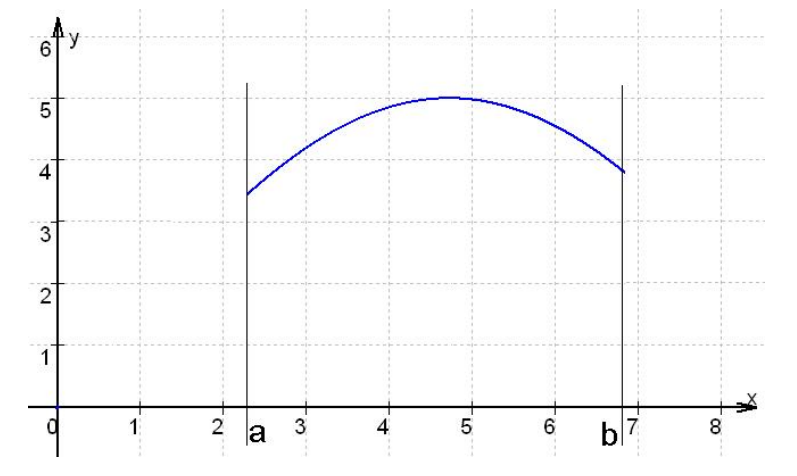
\includegraphics[width=8cm]{Bilder/keplersche_fassregel_funktion.png}
    \caption{Keplersche Fassregel \cite{skript}}    
    \label{fig:keplersche_fassregel}
\end{figure}
Wir betrachten eine Funktion $f$, deren Schaubild im gewünschten Intervall $I = [a, b]$ in \autoref{fig:sehnentrapeze_eins} gezeigt ist.

\begin{figure}[!tbp]
    \centering
    \begin{minipage}[b]{0.4\textwidth}
        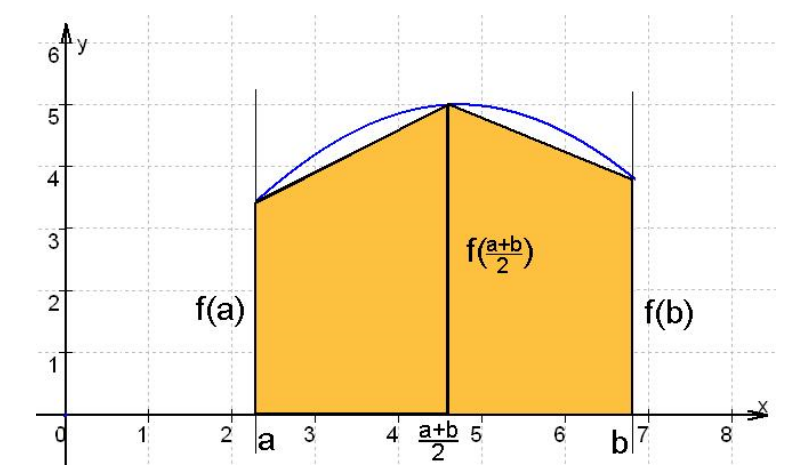
\includegraphics[width=8cm]{Bilder/sehnentrapeze.png}
      \caption{Sehnentrapeze für die anstehende Rechnung}
      \label{fig:sehnentrapeze_eins}
    \end{minipage}
    \hfill
    \begin{minipage}[b]{0.4\textwidth}
        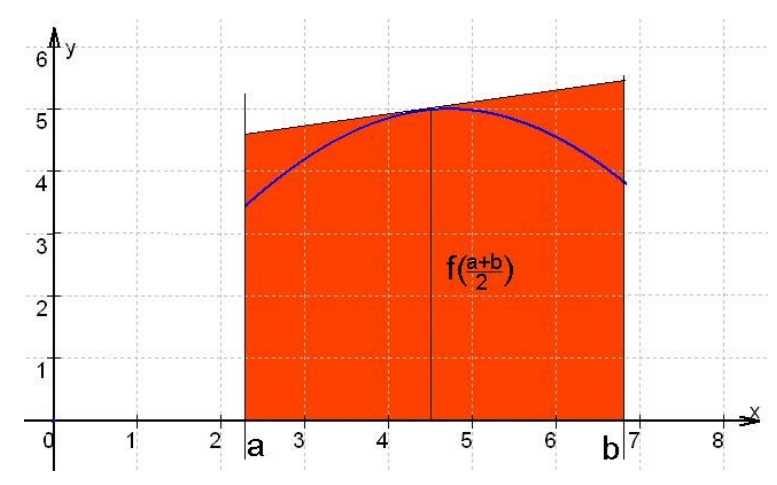
\includegraphics[width=8cm]{Bilder/sehnentrapez_addiert.png}
      \caption{Tangententrapez  \cite{skript}}
      \label{fig:sehnentrapeze_zwei}
    \end{minipage}
    \label{fig:sehnentrapeze}
  \end{figure}
\subsection*{A. Die zwei Sehnentrapeze}

Zur Flächenberechnung zeichnen wir zwei Sehnentrapeze in das gegebene Schaubild, wie in \autoref{fig:sehnentrapeze_eins} zu sehen ist. Für die Fläche eines Trapezes mit den Grundseiten $a$ und $b$ und der Höhe $h$ gilt:
\[
A_{\text{Trapez}} = \frac{a + b}{2} \cdot h = m \cdot h
\]
Übertragen auf die beiden Sehnentrapeze aus \autoref{fig:sehnentrapeze_eins} ergibt sich die Gesamtfläche $S$ als:
\[
S = \frac{b - a}{2} \cdot \left( \frac{f(a) + f\left( \frac{a + b}{2} \right)}{2} + \frac{f(b) + f\left( \frac{a + b}{2} \right)}{2} \right)
\]
\[
  \Leftrightarrow S = \frac{b - a}{2} \cdot \left(\frac{f(a)}{2} + f\left(\frac{a + b}{2}\right) + \frac{f(b)}{2}\right)
\]

\subsection*{B. Das Tangententrapez}

Nun legen wir ein weiteres Tangententrapez in das Schaubild, wie in \autoref{fig:sehnentrapeze_zwei} dargestellt. Nach der Trapezformel ergibt sich:
\[
T = f\left(\frac{a + b}{2}\right) \cdot (b - a)
\]
Da wir \textbf{doppelt so viele Sehnentrapeze wie Tangententrapeze} haben, gewichten wir die Flächen entsprechend. Die Gesamtfläche $I[f]$ nähert sich durch:
\[
I[f] \approx A = \frac{1}{3} \cdot (2S + T)
\]
\[
  \Leftrightarrow A = \frac{b - a}{6} \cdot \left(f(a) + 4 \cdot f\left(\frac{a + b}{2}\right) + f(b)\right)
\]

\subsection*{Die Keplersche Fassregel}

Ist die Funktion $f$ auf dem Intervall $I = [a, b]$ stetig, so gilt die Keplersche Fassregel:
\[
I[f] \approx A = \frac{b - a}{6} \cdot \left(f(a) + 4 \cdot f\left(\frac{a + b}{2}\right) + f(b)\right)
\]
Dabei ist zu beachten, dass die Keplersche Fassregel nur dann gute Näherungswerte liefert, wenn sich die Funktion im betrachteten Intervall durch eine Parabel annähern lässt (z.B. eine Normalverteilung). Daher ist es ratsam, das Intervall $[a, b]$ in \textbf{viele kleine, gleich große Teilintervalle} zu unterteilen und die Keplersche Fassregel auf jedes Teilintervall anzuwenden. Dabei sollte für eine bessere Genauigkeit das Intervall in möglichst viele, kleine Intervalle unterteilt werden. \cite{skript}

\subsection{Fehlerabschätzung}
\label{sec:fehlerabschätzung}

Für die Fehlerberechnung muss zunächst überhaupt definiert werden, was dieser Fehler ist:
\subsection*{Definition des Fehlers}
Der Fehler wird definiert als die Breite des Konfidenzintervalls:
\[
\text{Breite} = 2 \cdot c \cdot \frac{\sigma}{\sqrt{n}}
\]
Hierbei ist $c$ eine Konstante und wird mit der Trapezregel berechnet.

\subsection*{Berechnung des Standardfehlers}
Der Standardfehler (SE) des Mittelwerts wird berechnet als:
\[
SE = \frac{\sigma}{\sqrt{n}}
\]
Daraus folgt die Fehlerabschätzung:
\[
\text{Fehlerabschätzung} = c \cdot SE
\]
\subsection*{Interpretation}
Ein kleiner Fehler zeigt an, dass das Konfidenzintervall eine präzise Schätzung des wahren Mittelwerts bietet. Ein größerer Fehler deutet auf mögliche Unsicherheiten in den Daten oder eine unzureichende Stichprobengröße hin. Beispielsweise können so auch die Genauigkeit von Sensordaten oder ähnlichen eingeschätzt werden. 


\subsection{Vertrauensniveau $\gamma$}
\label{sec:vertrauensniveau}
Das Vertrauensniveau \(\gamma\) ist ein Wert, mit dem Angegeben wird wie sehr den Messwerte den wahren Wert des Parameters enthält (sprich wie genau die Sensoren sind). Es wird in der Regel als Dezimalzahl zwischen 0 und 1 dargestellt, wobei typische Werte 0.95 (95\%) und 0.99 (99\%) sind.

\begin{itemize}
    \item \textbf{Einfluss auf die Breite des Intervalls:} Ein höheres Vertrauensniveau führt zu einem breiteren Konfidenzintervall. Das bedeutet, dass wir mit größerer Sicherheit sagen können, dass der wahre Wert in diesem Intervall liegt. Ein niedrigeres Vertrauensniveau hingegen führt zu einem schmaleren Intervall, was die Schätzung präziser macht, aber auch das Risiko erhöht, dass der wahre Wert außerhalb liegt.
    
    \item \textbf{Berechnung:} Das Vertrauensniveau wird verwendet, um kritische Werte zu bestimmen, die notwendig sind, um das Konfidenzintervall zu berechnen. 
\end{itemize}

